\documentclass{article}
\title{Getting Started with LLGL}
\author{Lukas Hermanns}
\date{\today}

\usepackage{listings}
\usepackage{color}
\usepackage{pxfonts}
\usepackage{geometry}
\usepackage[T1]{fontenc}
\usepackage{xspace}
\usepackage{hyperref}
\usepackage{graphicx}
\usepackage{float}
\usepackage{pdfpages}

\geometry{
	a4paper,
	left=15mm,
	right=15mm,
	top=20mm,
	bottom=20mm
}

\begin{document}

\definecolor{brightBlueColor}{rgb}{0.5, 0.5, 1.0}
\definecolor{darkBlueColor}{rgb}{0.0, 0.0, 0.5}

\def\LLGL{\textcolor{darkBlueColor}{LLGL}\xspace}

\lstset{
	language = C++,
	basicstyle = \footnotesize\ttfamily,
	commentstyle = \itshape\color{brightBlueColor},
	keywordstyle = \bfseries\color{darkBlueColor},
	stringstyle = \color{red},
	frame = single,
	tabsize = 4,
	showstringspaces = false,
	numbers = none
}

\lstdefinelanguage{cmakeLanguage}
{
	morekeywords = {
		ADD_LIBRARY,
		SHARED,
		IF,
		ELSE,
		ELSEIF,
		ENDIF,
		FIND_PACKAGE,
		INCLUDE_DIRECTORIES,
		SET_TARGET_PROPERTIES,
		TARGET_LINK_LIBRARIES,
		TARGET_COMPILE_FEATURES,
		MESSAGE,
	},
	sensitive = false,
	morecomment = [l]{\#},
	morestring = [b]"
}

\maketitle

\begin{figure}[ht]
	\centering
	
\includegraphics[width=0.5\textwidth]{../LLGL_Logo.pdf}
\end{figure}

\newpage


%----------------------------------------------------------------------------------------
%	CONTENTS
%----------------------------------------------------------------------------------------

\tableofcontents

\newpage


%----------------------------------------------------------------------------------------
%	INTRRODUCTION
%----------------------------------------------------------------------------------------

\part{Introduction}


%----------------------------------------------------------------------------------------
%	IN A NUTSHELL
%----------------------------------------------------------------------------------------

\section{In a nutshell}

\subsection{What can \LLGL do for me?}

\begin{itemize}
	\item \textbf{Unification} \\
	\LLGL provides a unified interface across all supported renderers.
	Write your graphics render passes once and use them across multiple rendering APIs and platforms.
	
	\item \textbf{Low Overhead} \\
	\LLGL is meant to be a thin abstraction layer which only adds as less overhead between your application and the underlying rendering API as possible.
	At best, a function is just a wrapper that passes the parameters to the actual renderer.
	For example, the implementation of the \texttt{CommandBuffer::DrawIndexed} interface for Direct3D11:
\begin{lstlisting}
void D3D11CommandBuffer::DrawIndexed(std::uint32_t numVertices, std::uint32_t firstIndex) {
    context_->DrawIndexed(numVertices, firstIndex, 0);
}
\end{lstlisting}
	
	\item \textbf{Compatibility} \\
	\LLGL provides various compatibility functionalities between the renderers.
	For example, some image formats that are supported by OpenGL but not by Direct3D are converted `on the fly' by \LLGL.
	However, some compromises are inevitable, due to different hardware restrictions.
	All incompatibilities are well documented though.
	
	\item \textbf{Simplification} \\
	Where close access to the hardware is not necessary, \LLGL provides useful simplifications.
	For example, creating a render context as well as a device context across multiple platforms requires a lot of work when done manually.
	With \LLGL, this can be done with a few lines of code, but still have plenty of control thanks to the rich descriptor structures.
	
	\item \textbf{Debug Layer} \\
	In debug mode, \LLGL makes use of the native debug layers for the respective renderer.
	These debug layers, however, vary in quality depending on the API.
	\LLGL offers another debug layer on top of it that can be easily enabled or disabled.
	This layer performs state validation, parameter checks, warnings and errors messages before each draw call.
	This can be a powerful tool to find invalid render states or erronous descriptors.
	
	\item \textbf{Extension Support} \\
	Especially OpenGL is a complex system due to its many extensions.
	For texturing alone, \LLGL manages eight different extensions.
	Depending on which extension is available on the host platform, \LLGL uses the most efficient or otherwise emulates the functionality.
	Even a few vendor specific extensions are supported.
\end{itemize}


\subsection{What can \LLGL \emph{not} do for me?}

\begin{itemize}
	\item \textbf{Shader Cross Compilation} \\
	\LLGL unifies the underlying rendering APIs as far as possible, but since each rendering API has its own shading language,
	all shaders need to be provided for each desired renderer explicitly by the user.
	That said, there are several shader cross compilers available:
	\begin{itemize}
	\item XShaderCompiler (\href{https://github.com/LukasBanana/XShaderCompiler}{github.com/LukasBanana/XShaderCompiler}),
	\item SPIRV-Cross (\href{https://github.com/KhronosGroup/SPIRV-Cross}{github.com/KhronosGroup/SPIRV-Cross}),
	\item hlsl2glsl (\href{https://github.com/aras-p/hlsl2glslfork}{github.com/aras-p/hlsl2glslfork}).
	\item HLSLCrossCompiler (\href{https://github.com/James-Jones/HLSLCrossCompiler}{github.com/James-Jones/HLSLCrossCompiler})
	\end{itemize}
	
	\item \textbf{Scene Management} \\
	\LLGL is a low-level render system which does not provide any high-level scene management or animation system.
	It provides you with a set of functions to submit draw commands and render states to the graphics hardware as well as managing raw hardware buffers.
	`Game engine'-like functionality or anything beyond graphics is not part of \LLGL.
\end{itemize}


%----------------------------------------------------------------------------------------
%	PREREQUISITES
%----------------------------------------------------------------------------------------

\newpage
\section{Prerequisites}

\LLGL (Low Level Graphics Library) is a thin abstraction layer for graphics APIs such as
OpenGL, Direct3D, and Vulkan. It is meant to abstract these rendering technologies to one uniform interface.
The library is written entirely in C++11, so you'll
need a modern C++ compiler, i.e. at least \textbf{VisualC++ 2015} for Windows,
\textbf{g++ 4.8} for Linux, or \textbf{Clang 3.1} for MacOS.
To work with this library you should be familiar with these subjects:
\begin{itemize}
	\item \textbf{Basic C++11 Programming} \\
	Since the library is written in C++11, you should know something about \emph{smart pointers},
	\emph{raw pointers}, and basic \emph{object-oriented programming} (OOP) in C++.
	
	\item \textbf{Basic Linear Algebra} \\
	You should be familiar with at least \emph{Vectors} and \emph{Matrices}.
	
	\item \textbf{Fundamentals in Graphics Programming} \\
	You should be familiar with the fundamentals of graphics programming, since this is only a low-level graphics library.
	You should also be familiar with at least one of the major graphics APIs,
	i.e. \emph{OpenGL}, \emph{Direct3D}, \emph{Vulkan}, or \emph{Metal},
	because \LLGL does only little to no higher abstractions.
	
	\item \textbf{Shading Languages} \\
	\LLGL forces you to always write your own shaders, so you should be familiar with
	\href{https://www.opengl.org/documentation/glsl/}{GLSL} or
	\href{https://docs.microsoft.com/en-us/windows/desktop/direct3dhlsl/dx-graphics-hlsl}{HLSL}.
\end{itemize}


%----------------------------------------------------------------------------------------
%	PROGRESS
%----------------------------------------------------------------------------------------

\newpage
\section{Progress}

This project is still in its early steps. Here is a short overview of its progress:

\subsection{Platforms}
\begin{itemize}
	\item \textbf{Windows} \\
	Windows 10 is the main development environment of the author, so this platform has the best support.
	
	\item \textbf{MacOS} \\
	The MacOS port is in its early steps, but a few tutorials are already running.
	The development environment for the MacOS port is \emph{macOS Sierra}.
	
	\item \textbf{Linux} \\
	Ubuntu 17 (GNU/Linux) is used by the author to develop the linux port. GNU/Linux is supported for the most part.
	Both OpenGL and the Vulkan back-end are available.
\end{itemize}
	
\subsection{Renderers}
\begin{itemize}
	\item \textbf{OpenGL} \\
	OpenGL renderer is almost done (\textasciitilde 90\% complete).
	
	\item \textbf{Direct3D 11} \\
	Direct3D 11 renderer is almost done (\textasciitilde 90\% complete).
	
	\item \textbf{Direct3D 12} \\
	Direct3D 12 renderer is only in an experimental state (\textasciitilde 15\% complete).
	
	\item \textbf{Vulkan} \\
	Vulkan renderer is under heavy construction (\textasciitilde 30\% complete).
	
	\item \textbf{Metal} \\
	Metal renderer is only in an experimental state (\textasciitilde 5\% complete)..
\end{itemize}


%----------------------------------------------------------------------------------------
%	BUILD PROCESS
%----------------------------------------------------------------------------------------

\newpage
\section{Build Process}

\subsection{Cloning Repository}

There are some submodules in the \LLGL repository, all of which are optional though.
These submodules are located in the \texttt{external/} directory.
To clone the repository with \href{https://git-scm.com/}{git}, enter the following line in a command prompt:
\begin{lstlisting}[language=sh]
git clone https://github.com/LukasBanana/LLGL.git
\end{lstlisting}
To clone the repository with all its submodules, enter the following:
\begin{lstlisting}[language=sh]
git clone --recursive https://github.com/LukasBanana/LLGL.git
\end{lstlisting}

\subsection{Dependencies}

Since version 0.02, LLGL has no longer any required base dependencies except the one for the repsective renderers.
Previously, the \href{https://github.com/LukasBanana/GaussianLib}{\textsc{GaussianLib}} was required but has been replaced by a few plain-old-data structures.
The GaussianLib is now only required for the Examples and Test projects.

\subsubsection{OpenGL}

To build the OpenGL render system you need the OpenGL extension header files and an up-to-date graphics driver.
For Windows the header files \texttt{glext.h} and \texttt{wglext.h} are required.
For Linux the header files \texttt{glext.h} and \texttt{glxext.h} are required.
For MacOS no header files need to be downloaded, since the OpenGL version depends on the OS version.
You can find the header files at the \href{https://www.opengl.org/registry/#headers}{OpenGL registry page}.
Place the header files in the \texttt{include/GL/} folder of your compiler environment
or add the include path later in your build settings.

\subsubsection{Direct3D}

Since VisualStudio 2013, the DirectX framework (of which Direct3D is a part of) is included within
the VisualStudio setup, so no further SDK needs to be installed.

\subsubsection{Vulkan}

To build the Vulkan render system you need the \href{https://lunarg.com/vulkan-sdk/}{Vulkan SDK},
and of course a graphics driver which supports at least Vulkan 1.0.

\newpage
\subsection{Build Tool}

To build the \LLGL project files you need the build tool \href{https://cmake.org/}{CMake 2.8} or later.
The build process is now demonstrated with the CMake GUI on Windows, but it can also be configured
on a command line (more about this see \href{https://cmake.org/runningcmake/}{cmake.org/runningcmake}).

Set the source directory (``Where is the source code:'') to the \LLGL repository
and set the build directory (``Where to build the binaries'') where you want your project files.
In this example (see Figure \ref{fig:cmake_mask1}) the source directory is \texttt{<\dots>/LLGL/repository}
and the build directory is \texttt{<\dots>/LLGL/build\_msvc14} because the project files are build
for MSVC14 (VisualStudio 2015).

Now set the \textsc{GaussianLib} include directory (in this example \texttt{<...>/GaussianLib/repository/include})
and click on ``Configure''. If everything worked quite well, you should see the message ``Configuring done''
in the lower box. To finally create the project files, click on ``Generate''.
Then your project files should be located in the build directory you just set up previously.

\begin{figure}[ht]
	\centering
	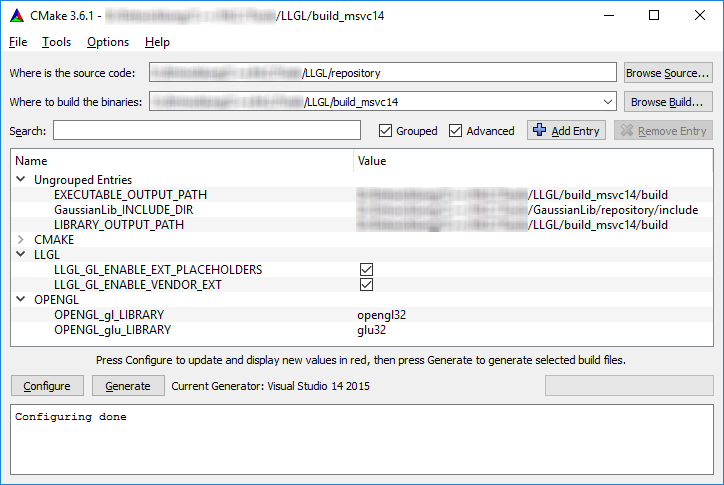
\includegraphics[width=0.85\textwidth]{cmake_mask1}
	\caption{CMake GUI mask to set up the project files for VisualStudio 2015 (MSVC14).}
	\label{fig:cmake_mask1}
\end{figure}

There are several options you can enable or disable to build the project:
\begin{itemize}
	\item \texttt{LLGL\_BUILD\_(TESTS/EXAMPLES/RENDERER\_\dots)} \\
	Specifies whether to include all test, all examples, or the repsective renderer projects.
	
	\item \texttt{LLGL\_D3D11\_ENABLE\_FEATURELEVEL} \\
	Specifies which feature level is enabled in the Direct3D 11 renderer.
	For example, feature level 11.1 requires that your development environment can find the \texttt{<d3d11\_1.h>} header file.
	Feature level 11.1 enables logic fragment operations, and feature level 11.3 enables conservative rasterization for the D3D11 renderer.
	
	\item \texttt{LLGL\_ENABLE\_CHECKED\_CAST} \\
	Specifies whether to enable or disable dynamic checked casts.
	This is only available in debug mode.
	
	\item \texttt{LLGL\_ENABLE\_DEBUG\_LAYER} \\
	Specifies whether to enable or disable the debug layer.
	This is a wrapper around the render system and all other render objects for effective debugging.
	
	\item \texttt{LLGL\_ENABLE\_SPIRV\_REFLECT} \\
	Specifies whether to include the submodule \texttt{external/SPIRV} to enable code reflection of SPIR-V shader modules for the Vulkan renderer.
	
	\item \texttt{LLGL\_ENABLE\_UTILITY} \\
	Specifies whether to enable or disable utility functions, which can be used to easily initialize descriptor structures.
	They must be included separately with the \texttt{LLGL/Utility.h} header file.
	
	\item \texttt{LLGL\_GL\_ENABLE\_DSA\_EXT} \\
	Specifies whether to enable or disable the \texttt{GL\_ARB\_direct\_state\_access} extension that spans the entire render system.
	
	\item \texttt{LLGL\_GL\_ENABLE\_EXT\_PLACEHOLDERS} \\
	Specifies whether OpenGL extensions should be replaced by placeholder procedures
	when they are not available. This may help debugging and should not influence the runtime performance.
	
	\item \texttt{LLGL\_GL\_ENABLE\_VENDOR\_EXT} \\
	Specifies whether vendor specific OpenGL extensions should be enabled or disabled.
	One of these extensions is for conservative rasterization
	(\texttt{GL\_NV\_conservative\_raster} and \texttt{GL\_INTEL\_conservative\_rasterization}) for instance.
	These extensions will only be loaded and used by the runtime if they are available on the host platform.
	
	\item \texttt{LLGL\_GL\_INCLUDE\_EXTERNAL} \\
	Specifies whether to include the OpenGL header files from the \texttt{external/GL/} directory of the LLGL repository.
	Otherwise the \texttt{GL/} directory must be elsewhere specified in your include search paths.
\end{itemize}


%----------------------------------------------------------------------------------------
%	API OVERVIEW
%----------------------------------------------------------------------------------------

\clearpage
\newpage
\section{API Overview}

LLGL has a very simple and unified API design.
For object creation, there is commonly a ``\texttt{\dots Descriptor}'' structure (e.g. \texttt{LLGL::BufferDescriptor}),
which contains all necessary information to describe the object which is to be created.

\subsection{Rendering Interfaces}

There are three major interfaces for rendering:
\emph{RenderSystem} is mainly used for object creation and memory read/write operations,
\emph{RenderContext} is used to configure each framebuffer and its back buffer (or rather swap chain),
and \emph{CommandBuffer} which is used to set render states, draw primitives, and dispatch compute commands.

\subsubsection{RenderSystem}

In the \texttt{RenderSystem} interface there are several functions of the following form:
\begin{lstlisting}
// Create a new object
Create...

// Update the data of an object
Write...

// Read the data from an object
Read...

// Map the memory of an object from GPU to CPU memory space
Map...

// Unmap the memory from an object
Unmap...

// Release an object
Release
\end{lstlisting}

\subsubsection{RenderContext}

The most important function in the \texttt{RenderContext} interface is \texttt{Present},
to show the content of the back buffer on the screen.
There are a few other functions to access the context window and change the video mode:
\begin{lstlisting}
// Access context surface (this is the window on desktop platforms).
GetSurface

// Set video mode (i.e. resolution, fullscreen/windowed mode etc.)
SetVideoMode

// Set vertical synchronization (Vsync) for swap-chain
SetVsync
\end{lstlisting}

\subsubsection{CommandBuffer}

There are several overloaded functions for drawing operations with the naming convention
``\texttt{Draw}'', ``\texttt{DrawIndexed}'', ``\texttt{DrawInstanced}'', or ``\texttt{DrawIndexedInstanced}''.
The most other functions are used to configure the command buffer of the graphics API, which have the following form:
\begin{lstlisting}
// Set a hardware buffer/ texture/ sampler etc.
Set...

// Begin and always end a state (e.g. BeginQuery/ EndQuery)
Begin...
End...

// Draw primitives
Draw...
\end{lstlisting}

\subsection{Windowing System}

LLGL has the \texttt{Window} interface for a very basic but platform independent windowing system.
Use its static function \texttt{Create} to create an instance of this interface for the host platform.
A custom implementation of this interface can also be written and used for any renderer.
In section \ref{sec:custom_surface} an example of a custom implementation with \href{http://www.glfw.org/}{GLFW} is shown.


%----------------------------------------------------------------------------------------
%	HELLO TRIANGLE
%----------------------------------------------------------------------------------------

\newpage
\part{Tutorials}

\section{Hello Triangle}

\textit{NOTE: this section is not up-to-date!} \\
\noindent

After we have set up and build the library, we can start rendering some geometry.
Our example will consist of a single C++ source file (e.g. ``\texttt{main.cpp}'') and two shader files
(e.g. ``\texttt{vertex.glsl}'' and ``\texttt{fragment.glsl}'').
The include path for a project, that uses \LLGL, must be set to \texttt{\textit{<your-LLGL-repository>}/include/},
and the \LLGL library file must be added to the linker (for Windows this is ``\texttt{LLGL.lib}''
when compiling in Release mode and ``\texttt{LLGLD.lib}'' when compiling in Debug mode).
All the other library files don't need to be added to the linker (e.g. ``\texttt{LLGL\_OpenGL.lib}''),
since the respective renderer module is loaded at runtime.

Now let's start with a small example. At first we need to include the header files.
The main header we need is \texttt{LLGL/LLGL.h} where the entire \LLGL interface is declared.
For our example we also need basic I/O classes from \texttt{iostream} for standard output, \texttt{fstream}
to read the shader files, and \texttt{Gauss/Gauss.h} for some matrix classes:
\begin{lstlisting}
#include <LLGL/LLGL.h>
#include <Gauss/Gauss.h>
#include <iostream>
#include <fstream>
\end{lstlisting}
Next we define the C++ main function and wrap the entire example code into a large \texttt{try-catch} block,
to quit the application with a meaningful error message if any failure happens:
\begin{lstlisting}
int main() {
    try {
        /* example code here ... */
    } catch (const std::exception& e) {
        std::cerr << e.what() << std::endl;
    }
    return 0;
}
\end{lstlisting}
To create an \LLGL renderer instance in our main function, we load a renderer module
(a \textit{module} here denotes a dynamic shared library)
from the static \texttt{Load} function of the \texttt{RenderSystem} interface:
\begin{lstlisting}
std::unique_ptr<LLGL::RenderSystem> renderer = LLGL::RenderSystem::Load("OpenGL");
\end{lstlisting}
Here we could actually use the C++11 keyword \texttt{auto} to simplify the code,
but for explanation purposes we keep the types explicit.
Most creation or load functions return a new instance wrapped in a \texttt{std::unique\_ptr},
but in this case \LLGL needs to keep track of the instance to check if it has already been expired,
which is only feasible with an \texttt{std::shared\_ptr}.

Moreover, most functions use enumerations instead of strings to specify some type, but in this case
a module can be loaded dynamically at runtime and further modules can be added or removed independently.
Therefore the renderer module is specified by a string (here ``OpenGL''). Other modules are
named ``Direct3D11'', ``Direct3D12'', and ``Vulkan''.
Whenver you load a new renderer, there must not remain any references to this shared object,
because only a single renderer can be loaded at a time.
When this shared object expires, all objects allocated by this renderer will be deleted automatically.

If loading the renderer failed, an \texttt{std::runtime\_error} exception will be thrown,
which can be cached to show an error message and/or load another renderer module instead.
This can be very handy if a specific Direct3D version is not installed on the host Windows platform,
so another Direct3D version or OpenGL renderer can be loaded as fallback
without disturbing the user with akward error messages and program crashes.

After we created the renderer we need a graphics context to draw into.
This is done by the \texttt{CreateRenderContext} function which takes a descriptor structure:
\begin{lstlisting}
LLGL::RenderContextDescriptor contextDesc;
{
    contextDesc.videoMode.resolution = { 640, 480 };
}
LLGL::RenderContext* context = renderer->CreateRenderContext(contextDesc);
\end{lstlisting}
This is a minimal example for the render context descriptor. There are much more attributes
to specify multi-sampled anti-aliasing, vertical-synchronisation, etc.
See the API documentation for more information about these attributes.

This render context will create its own window, but we could also specifiy our own one.
However, in this example we keep it simple. To access this window and change the title,
we use the \texttt{GetWindow} function of the \texttt{RenderContext} interface
which returns a reference to its window:
\begin{lstlisting}
context->GetWindow().SetTitle(L"LLGL Tutorial 01: Hello Triangle");
\end{lstlisting}
Since some platforms (such as Win32) support Unicode window titles, our string literal starts with the `L' token.

Next we create a vertex buffer to store our geometry. For this example we give up an index buffer,
since we only draw a single triangle and no complex models. At first we define our vertex data and the vertex format,
which is required to tell the rendering API how the vertex attributes are located within the vertex buffer:
\begin{lstlisting}
// Vertex data structure
struct Vertex {
    Gs::Vector2f    position;
    LLGL::ColorRGBf color;
};

// Vertex data (3 vertices for our triangle)
Vertex vertices[] = {
    { {  0,  1 }, { 1, 0, 0 } }, // 1st vertex: center-top, red
    { {  1, -1 }, { 0, 1, 0 } }, // 2nd vertex: right-bottom, green
    { { -1, -1 }, { 0, 0, 1 } }, // 3rd vertex: left-bottom, blue
};

// Vertex format
LLGL::VertexFormat vertexFormat;
vertexFormat.AppendAttribute({ "position", LLGL::VectorType::Float2 }); // position has 2D float vector
vertexFormat.AppendAttribute({ "color",    LLGL::VectorType::Float3 }); // color has 3D float vector
\end{lstlisting}
The \texttt{AppendAttribute} function adds the attributes to the vertex format.
The order of these function calls determines the location in the vertex data, so they must match
the order of the member fields in the vertex data structure (here ``\texttt{struct Vertex}'').

Now we can create our vertex buffer and upload the vertex data to the GPU by passing a pointer
to the \texttt{initialData} parameter:
\begin{lstlisting}
LLGL::BufferDescriptor bufferDesc;

// Define size (in bytes) of the buffer
bufferDesc.size = sizeof(vertices);

// We will bind it as a vertex buffer (can be a bitwise OR combination)
bufferDesc.bindFlags = LLGL::BindFlags::VertexBuffer;

// Set vertex buffer specific attributes
bufferDesc.vertexBuffer.format = vertexFormat; // Copy the vertex format

LLGL::Buffer* vertexBuffer = renderer->CreateBuffer(bufferDesc, vertices);
\end{lstlisting}
To update an entire hardware buffer or texture (or only a portion of it) there is a respective
``\texttt{Write...}'' function.

Now we have the vertex buffer complete and we can cross over to shader creation.
In \LLGL the shaders (Vertex, Tessellation-Control, Tessellation-Evaluation, Geometry, Fragment, and Compute shaders)
are created independently, and then attached and linked together with a shader program.
For our example we only need a Vertex- and Fragment (also called ``Pixel'') shader:
\begin{lstlisting}
LLGL::Shader* vertexShader = renderer->CreateShader(LLGL::ShaderType::Vertex);
LLGL::Shader* fragmentShader = renderer->CreateShader(LLGL::ShaderType::Fragment);
\end{lstlisting}
Now we have two empty shaders. Next we load the shader code from file with
our custom ``\texttt{ReadFileContent}'' lambda function:
\begin{lstlisting}
// Define the lambda function to read an entire text file
auto ReadFileContent = [](const std::string& filename) {
    std::ifstream file(filename);
    return std::string( ( std::istreambuf_iterator<char>(file) ),
                        ( std::istreambuf_iterator<char>(    ) ) );
};

// Load vertex- and fragment shader code from file
std::string vertexShaderCode = ReadFileContent("vertex.glsl");
std::string fragmentShaderCode = ReadFileContent("fragment.glsl");
\end{lstlisting}

After reading the shader code into strings we can compile the shaders:
\begin{lstlisting}
auto CompileShader = [](LLGL::Shader* shader, const std::string& code) {
    // Compile shader
    shader->Compile(code);
    
    // Print info log (warnings and errors)
    std::string log = shader->QueryInfoLog();
    if (!log.empty()) {
        std::cerr << log << std::endl;
    }
};

CompileShader(vertexShader, vertexShaderCode);
CompileShader(fragmentShader, fragmentShaderCode);
\end{lstlisting}
Shader compilation works a little different between GLSL (for OpenGL) and HLSL (for Direct3D).
For HLSL shader compilation there is a second overloaded ``\texttt{Compile}'' function with more parameters,
to specifiy the entry point and shader version target.

Having the shaders compiled, we can now create a shader program, attach all shaders to it,
bind the vertex attribute layout, and finally link the shader program:
\begin{lstlisting}
// Create shader program which is used as composite
LLGL::ShaderProgram* shaderProgram = renderer->CreateShaderProgram();

// Attach vertex- and fragment shader to the shader program
shaderProgram->AttachShader(*vertexShader);
shaderProgram->AttachShader(*fragmentShader);

// Build vertex layout for input assembly (this is not required for a compute shader program).
// Multiple vertex formats can be passed when the vertex data comes from multiple vertex buffers.
shaderProgram->BuildInputLayout(1, &vertexFormat);

// Link shader program and check for errors
if (!shaderProgram->LinkShaders()) {
    throw std::runtime_error(shaderProgram->QueryInfoLog());
}
\end{lstlisting}
The ``\texttt{BuildInputLayout}'' function binds the vertex attributes to the shader program.
This must be called after shader attachment but before shader linking (except a compute shader program is used).

Before we continue with the C++ code, we first take a look at the shader code:
\begin{lstlisting}[title={\texttt{vertex.glsl}}]
// GLSL shader version 1.30 (for OpenGL 3.1)
#version 130

// Vertex attributes (these names must match our vertex format attributes)
in vec2 position;
in vec3 color;

// Vertex output to the fragment shader
out vec3 vertexColor;

// Vertex shader main function
void main() {
    gl_Position = vec4(position, 0, 1);
    vertexColor = color;
}
\end{lstlisting}
This simple vertex shader only passes the vertex position and color (with default interpolation) to the fragment shader.
And here is the fragment shader:
\begin{lstlisting}[title={\texttt{fragment.glsl}}]
// GLSL shader version 1.30 (for OpenGL 3.1)
#version 130

// Fragment input from the vertex shader
in vec3 vertexColor;

// Fragment output color
out vec4 fragColor;

// Fragment shader main function
void main() {
    fragColor = vec4(vertexColor, 1);
}
\end{lstlisting}

Now we are finally done with setting up the shader. Next we need to create a graphics pipeline.
This concept is derived from modern graphics APIs such as Direct3D 12 and Vulkan.
The major pipeline state is stored inside this pipeline state object.
For older graphics APIs (such as OpenGL) \LLGL will set the respective render states by its internal state manager,
to reduce state changes.

The graphics pipeline specifies the depth-, stencil-, rasterizer-, blending-,
and shader states and is created as follows:
\begin{lstlisting}
LLGL::GraphicsPipelineDescriptor pipelineDesc;
{
    pipelineDesc.shaderProgram = shaderProgram;
}
LLGL::GraphicsPipeline* pipeline = renderer->CreateGraphicsPipeline(pipelineDesc);
\end{lstlisting}
In our example we can use all default settings of the graphics pipeline descriptor except the shader program,
which must always be set by the client programmer.

Before we start with the render main loop, we need a command buffer which can send render state and draw commands to the GPU:
\begin{lstlisting}
// Create command buffer to submit subsequent graphics commands to the GPU
LLGL::CommandBuffer* commands = renderer->CreateCommandBuffer();
\end{lstlisting}
We now have all render objects, so we can start with the main loop:
\begin{lstlisting}
// Run main loop until the main window is closed
while (context->GetWindow().ProcessEvents()) {
    /* render code here ... */
}
\end{lstlisting}
This main loop will run until the user clicks the close button on the window of the render context.
The rest of the code is pretty simple, since the most work is done during initialization.
What we need to do is to clear the color buffer of the previous frame,
set the graphics pipeline, set the vertex buffer, draw the primitives, and present the result on the frame buffer:
\begin{lstlisting}
// Set the render context as the initial render target
commands->SetRenderTarget(*context);

// Set viewport (left: 0, top: 0, width: 640, height: 480)
commands->SetViewport({ 0, 0, 640, 480 });

// Clear color buffer
commands->Clear(LLGL::ClearFlags::Color);

// Bind graphics pipeline
commands->SetGraphicsPipeline(*pipeline);

// Bind vertex buffer
commands->SetVertexBuffer(*vertexBuffer);

// Generate 3 vertices to draw a triangle
commands->Draw(3, 0);

// Present the result on the frame buffer (or rather on the screen)
context->Present();
\end{lstlisting}
When you have done everything right, you should see something like shown in figure \ref{fig:tut01_mask1} after compilation
and program start (set working directory to \texttt{tutorial/Tutorial01\_HelloTriangle}).
\begin{figure}[H]
	\centering
	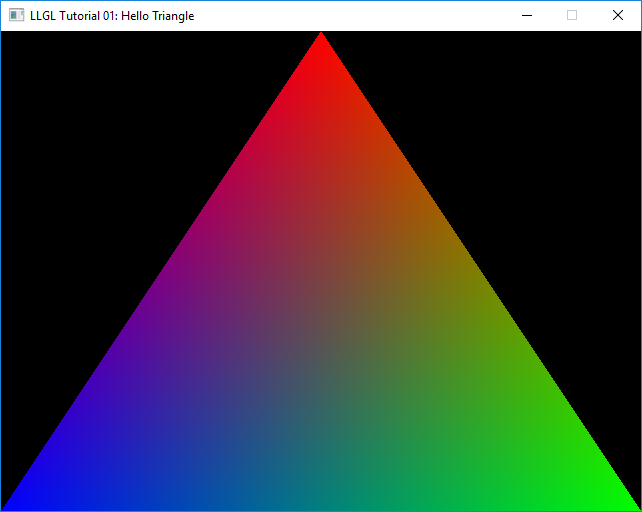
\includegraphics[width=0.9 \textwidth]{tut01_mask1a}
	\caption{Output of the ``Tutorial01: HelloTriangle'' running on Windows 10.}
	\label{fig:tut01_mask1}
\end{figure}


%----------------------------------------------------------------------------------------
%	CUSTOM WINDOW CLASS
%----------------------------------------------------------------------------------------

\newpage
\part{Extensibility}

\section{Custom Surface Class}
\label{sec:custom_surface}

In this example a simple custom implementation of the \texttt{Surface} interface is demonstrated,
to show how LLGL can be used with other windowing system libraries.
Here we will use the popular cross-platform library \href{http://www.glfw.org/}{GLFW}.

We start with the include files of GLFW and LLGL:
\begin{lstlisting}
// Include GLFW library (in this example we use the Win32 platform)
#define GLFW_EXPOSE_NATIVE_WIN32
#include <GLFW/glfw3.h>
#include <GLFW/glfw3native.h>

// Include LLGL and also the native handle structures
#include <LLGL/LLGL.h>
#include <LLGL/Platform/NativeHandle.h>
\end{lstlisting}
Now we declare our custom surface class and override all necessary interface functions.
We could also inherit from the \texttt{Window} interface but this is not really meaningful here:
\begin{lstlisting}
class CustomSurface : public LLGL::Surface
{
public:
	// Constructor and destructor
	CustomSurface(const LLGL::Extent2D& size, const std::string& title);
	~CustomSurface();
	
	// Interface implementation
	void GetNativeHandle(void* nativeHandle) const override;
	LLGL::Extent2D GetContentSize() const override;
	bool AdaptForVideoMode(LLGL::VideoModeDescriptor& videoModeDesc) override;
	void ResetPixelFormat() override;
	
	// Additional class functions
	void PollEvents();
	
private:
	GLFWwindow* CreateGLFWWindow();
	
	std::string    title_;
	LLGL::Extent2D size_;
	GLFWwindow* wnd_ = nullptr; // GLFW window pointer
	
};
\end{lstlisting}
This is an example of a minimal interface implementation.
We start implementing the constructor, destructor, and the \texttt{CreateGLFWWindow} function:
\begin{lstlisting}
CustomSurface::CustomSurface(const LLGL::Extent2D& size, const std::string& title) :
	title_ { title              },
	size_  { size               },
	wnd_   { CreateGLFWWindow() }
{
}

CustomSurface::~CustomSurface()
{
	// Destroy GLFW window
	glfwDestroyWindow(wnd_);
}

GLFWwindow* CustomSurface::CreateGLFWWindow()
{
	// Create GLFW window with class members
	auto wnd = glfwCreateWindow(size_.width, size_.height, title_.c_str(), nullptr, nullptr);
	if (!wnd)
		throw std::runtime_error("failed to create GLFW window");
	return wnd;
}
\end{lstlisting}
Now we cross over to the major functions in the \texttt{Surface} interface. The first one is \texttt{ResetPixelFormat}.
It is mainly used by the OpenGL renderer when a multi-sampled render context is created on Win32.
In our custom class we merely destroy the GLFW window and create a new one.
It's the only way on Win32 to reset the internal pixel format of the native window object:
\begin{lstlisting}
void CustomSurface::ResetPixelFormat()
{
	// Destroy and recreate GLFW window
	glfwDestroyWindow(wnd_);
	wnd_ = CreateGLFWWindow();
}
\end{lstlisting}
Next we implement the \texttt{GetNativeHandle} function. This is also very important,
because any renderer needs access to the native window handle.
On MS/Windows this is from the type \texttt{HWND} from the Win32 API.
On GNU/Linux we need to pass three parameters: \texttt{Display*} from the X11 lib,
\texttt{::Window} from the X11 lib (unfortunately the same name but in the global scope),
and \texttt{XVisualInfo*} from GLX.
On MacOS it is from the type \texttt{NSWindow*} from the Cocoa API.
In this example we only implement it for Win32:
\begin{lstlisting}
void CustomSurface::GetNativeHandle(void* nativeHandle) const
{
	// This function must always return a valid native handle!
	auto handle = reinterpret_cast<LLGL::NativeHandle*>(nativeHandle);
	handle->window = glfwGetWin32Window(wnd_);
}
\end{lstlisting}
There are two (rather secondary) interface functions left.
They are used inside the \texttt{RenderContext} class, to update or query the video mode suitable for the surface:
\begin{lstlisting}
LLGL::Extent2D CustomSurface::GetContentSize() const
{
	// Actually the client-area size of the window must be returned,
	// but for this example the entire window size is sufficient.
	return size_;
}

bool CustomSurface::AdaptForVideoMode(LLGL::VideoModeDescriptor& videoModeDesc)
{
	// Resize GLFW window for the new video mode resolution.
	size_ = videoModeDesc.resolution;
	glfwSetWindowSize(wnd_, size_.width, size_.height);
	return true;
}
\end{lstlisting}
The last function we have to implement is the additional class function \texttt{PollEvents}.
Here we poll all window events from GLFW and return false when the user
clicked the close button to terminate the application:
\begin{lstlisting}
bool CustomSurface::PollEvents()
{
	// Poll events from GLFW windowing system
	glfwPollEvents();
	
	// Return true until the user pressed the close button
	return !glfwWindowShouldClose(wnd_);
}
\end{lstlisting}
Finally we are done with our custom window class :-) Now we can start using it with a render context in our main function:
\begin{lstlisting}
// Initialize GLFW
if (!glfwInit())
	return -1;

// Create an instance of our custom window class
auto surface = std::make_shared<CustomSurface>({ 640, 480 }, L"LLGL test with GLFW");

// Create render context and pass the custom window
LLGL::RenderContextDescriptor contextDesc;
contextDesc.videoMode.resolution = { 640, 480 };
LLGL::RenderContext* context = renderer->CreateRenderContext(contextDesc, surface);

// Scene construction ...

while (surface->PollEvents()) { /* Rendering ... */ }
\end{lstlisting}
That's all folks. The rest can be seen in the tutorials.


%----------------------------------------------------------------------------------------
%	CUSTOM RENDER SYSTEM
%----------------------------------------------------------------------------------------

\newpage
\section{Custom Render System}
\label{sec:custom_renderer}

This is only a very short explanation on how to implement your own render system with LLGL,
since it will take a lot of familiarization time anyways.

First of all you have to extend the \texttt{CMakeLists.txt} file in your local LLGL repository for a new library.
Here is an example on how it could look for a custom OpenGL renderer:
\begin{lstlisting}[language=cmakeLanguage]
# Find OpenGL headers and libraries
FIND_PACKAGE(OpenGL)

IF(OpenGL_FOUND)
	# Add OpenGL include path
	INCLUDE_DIRECTORIES(${OPENGL_INCLUDE_DIR})
	
	# Add "LLGL_CustomOpenGL" library project to the solution,
	# where "FilesGL" denotes the variable containing all filenames for this render system.
	# The render system can later be loaded with the name "CustomOpenGL".
	ADD_LIBRARY(LLGL_CustomOpenGL SHARED "${FilesGL}")
	
	# Add "D" postfix to debug mode (this is required so that LLGL loads the correct module)
	SET_TARGET_PROPERTIES(
		LLGL_CustomOpenGL PROPERTIES
		LINKER_LANGUAGE CXX # CXX is for C++
		DEBUG_POSTFIX "D" # Postfix "D" for debug mode
	)
	
	# Add library dependencies (On Win32 this is LLGL.lib and opengl32.lib)
	TARGET_LINK_LIBRARIES(LLGL_CustomOpenGL LLGL "${OPENGL_LIBRARIES}")
	
	# Tell CMake to build a project with C++11 support
	TARGET_COMPILE_FEATURES(LLGL_CustomOpenGL PRIVATE cxx_range_for)
ELSE()
	MESSAGE("Missing OpenGL -> LLGL_CustomOpenGL renderer will be excluded from project")
ENDIF()
\end{lstlisting}
After you integrated your source files into the LLGL project solution,
you have to implement a few module interface functions.
They are the only functions that need to be exported from the shared library,
and they need to be exported as \texttt{extern "C"} functions:
\begin{lstlisting}
// Include the "ModuleInterface.h" file and your custom render system
#include "sources/Renderer/ModuleInterface.h"
#include "CustomOpenGLRenderSystem.h"

// Declare the following functions to be exported as "C" functions
extern "C"
{

// This function must always return "LLGL_BUILD_ID" to ensure a library,
// which is about to be loaded, has been compiled with the same compiler toolchain.
LLGL_EXPORT int LLGL_RenderSystem_BuildID()
{
	return LLGL_BUILD_ID;
}

// Here you can return your own renderer ID or one of the pre-defined values
LLGL_EXPORT int LLGL_RenderSystem_RendererID(const void* renderSystemDesc)
{
	return LLGL::RendererID::OpenGL;
}

// Here you can return the name of your renderer
LLGL_EXPORT const char* LLGL_RenderSystem_Name(const void* renderSystemDesc)
{
	return "Custom OpenGL";
}

// Here you have to return a raw pointer of your custom implementation of the
// LLGL::RenderSystem interface, where the instance must be allocated with "new",
// so it can be moved into an std::unique_ptr.
LLGL_EXPORT void* LLGL_RenderSystem_Alloc(const void* renderSystemDesc)
{
	return new CustomOpenGLRenderSystem();
}

} // /extern "C"
\end{lstlisting}
That's all you have to do, except of implementing the entire \texttt{RenderSystem} interface
in your \texttt{CustomOpenGLRenderSystem} class ;-).
After that, you can load your render system like this:
\begin{lstlisting}
// Load custom render system (library name is "LLGL_CustomOpenGL", so the passed name is "CustomOpenGL")
std::unique_ptr<LLGL::RenderSystem> renderer = LLGL::RenderSystem::Load("CustomOpenGL");

// Start using the custom renderer ...
\end{lstlisting}


%----------------------------------------------------------------------------------------
%	APPENDIX
%----------------------------------------------------------------------------------------

%\newpage

%\section{Appendix}

%Foo bar ...






\end{document}
